% Options for packages loaded elsewhere
\PassOptionsToPackage{unicode}{hyperref}
\PassOptionsToPackage{hyphens}{url}
%
\documentclass[
]{article}
\usepackage{amsmath,amssymb}
\usepackage{lmodern}
\usepackage{iftex}
\ifPDFTeX
  \usepackage[T1]{fontenc}
  \usepackage[utf8]{inputenc}
  \usepackage{textcomp} % provide euro and other symbols
\else % if luatex or xetex
  \usepackage{unicode-math}
  \defaultfontfeatures{Scale=MatchLowercase}
  \defaultfontfeatures[\rmfamily]{Ligatures=TeX,Scale=1}
\fi
% Use upquote if available, for straight quotes in verbatim environments
\IfFileExists{upquote.sty}{\usepackage{upquote}}{}
\IfFileExists{microtype.sty}{% use microtype if available
  \usepackage[]{microtype}
  \UseMicrotypeSet[protrusion]{basicmath} % disable protrusion for tt fonts
}{}
\makeatletter
\@ifundefined{KOMAClassName}{% if non-KOMA class
  \IfFileExists{parskip.sty}{%
    \usepackage{parskip}
  }{% else
    \setlength{\parindent}{0pt}
    \setlength{\parskip}{6pt plus 2pt minus 1pt}}
}{% if KOMA class
  \KOMAoptions{parskip=half}}
\makeatother
\usepackage{xcolor}
\IfFileExists{xurl.sty}{\usepackage{xurl}}{} % add URL line breaks if available
\IfFileExists{bookmark.sty}{\usepackage{bookmark}}{\usepackage{hyperref}}
\hypersetup{
  pdftitle={BKN 599 - Final Exam},
  pdfauthor={FirstName LastName},
  hidelinks,
  pdfcreator={LaTeX via pandoc}}
\urlstyle{same} % disable monospaced font for URLs
\usepackage[margin=1in]{geometry}
\usepackage{color}
\usepackage{fancyvrb}
\newcommand{\VerbBar}{|}
\newcommand{\VERB}{\Verb[commandchars=\\\{\}]}
\DefineVerbatimEnvironment{Highlighting}{Verbatim}{commandchars=\\\{\}}
% Add ',fontsize=\small' for more characters per line
\usepackage{framed}
\definecolor{shadecolor}{RGB}{248,248,248}
\newenvironment{Shaded}{\begin{snugshade}}{\end{snugshade}}
\newcommand{\AlertTok}[1]{\textcolor[rgb]{0.94,0.16,0.16}{#1}}
\newcommand{\AnnotationTok}[1]{\textcolor[rgb]{0.56,0.35,0.01}{\textbf{\textit{#1}}}}
\newcommand{\AttributeTok}[1]{\textcolor[rgb]{0.77,0.63,0.00}{#1}}
\newcommand{\BaseNTok}[1]{\textcolor[rgb]{0.00,0.00,0.81}{#1}}
\newcommand{\BuiltInTok}[1]{#1}
\newcommand{\CharTok}[1]{\textcolor[rgb]{0.31,0.60,0.02}{#1}}
\newcommand{\CommentTok}[1]{\textcolor[rgb]{0.56,0.35,0.01}{\textit{#1}}}
\newcommand{\CommentVarTok}[1]{\textcolor[rgb]{0.56,0.35,0.01}{\textbf{\textit{#1}}}}
\newcommand{\ConstantTok}[1]{\textcolor[rgb]{0.00,0.00,0.00}{#1}}
\newcommand{\ControlFlowTok}[1]{\textcolor[rgb]{0.13,0.29,0.53}{\textbf{#1}}}
\newcommand{\DataTypeTok}[1]{\textcolor[rgb]{0.13,0.29,0.53}{#1}}
\newcommand{\DecValTok}[1]{\textcolor[rgb]{0.00,0.00,0.81}{#1}}
\newcommand{\DocumentationTok}[1]{\textcolor[rgb]{0.56,0.35,0.01}{\textbf{\textit{#1}}}}
\newcommand{\ErrorTok}[1]{\textcolor[rgb]{0.64,0.00,0.00}{\textbf{#1}}}
\newcommand{\ExtensionTok}[1]{#1}
\newcommand{\FloatTok}[1]{\textcolor[rgb]{0.00,0.00,0.81}{#1}}
\newcommand{\FunctionTok}[1]{\textcolor[rgb]{0.00,0.00,0.00}{#1}}
\newcommand{\ImportTok}[1]{#1}
\newcommand{\InformationTok}[1]{\textcolor[rgb]{0.56,0.35,0.01}{\textbf{\textit{#1}}}}
\newcommand{\KeywordTok}[1]{\textcolor[rgb]{0.13,0.29,0.53}{\textbf{#1}}}
\newcommand{\NormalTok}[1]{#1}
\newcommand{\OperatorTok}[1]{\textcolor[rgb]{0.81,0.36,0.00}{\textbf{#1}}}
\newcommand{\OtherTok}[1]{\textcolor[rgb]{0.56,0.35,0.01}{#1}}
\newcommand{\PreprocessorTok}[1]{\textcolor[rgb]{0.56,0.35,0.01}{\textit{#1}}}
\newcommand{\RegionMarkerTok}[1]{#1}
\newcommand{\SpecialCharTok}[1]{\textcolor[rgb]{0.00,0.00,0.00}{#1}}
\newcommand{\SpecialStringTok}[1]{\textcolor[rgb]{0.31,0.60,0.02}{#1}}
\newcommand{\StringTok}[1]{\textcolor[rgb]{0.31,0.60,0.02}{#1}}
\newcommand{\VariableTok}[1]{\textcolor[rgb]{0.00,0.00,0.00}{#1}}
\newcommand{\VerbatimStringTok}[1]{\textcolor[rgb]{0.31,0.60,0.02}{#1}}
\newcommand{\WarningTok}[1]{\textcolor[rgb]{0.56,0.35,0.01}{\textbf{\textit{#1}}}}
\usepackage{graphicx}
\makeatletter
\def\maxwidth{\ifdim\Gin@nat@width>\linewidth\linewidth\else\Gin@nat@width\fi}
\def\maxheight{\ifdim\Gin@nat@height>\textheight\textheight\else\Gin@nat@height\fi}
\makeatother
% Scale images if necessary, so that they will not overflow the page
% margins by default, and it is still possible to overwrite the defaults
% using explicit options in \includegraphics[width, height, ...]{}
\setkeys{Gin}{width=\maxwidth,height=\maxheight,keepaspectratio}
% Set default figure placement to htbp
\makeatletter
\def\fps@figure{htbp}
\makeatother
\setlength{\emergencystretch}{3em} % prevent overfull lines
\providecommand{\tightlist}{%
  \setlength{\itemsep}{0pt}\setlength{\parskip}{0pt}}
\setcounter{secnumdepth}{-\maxdimen} % remove section numbering
\ifLuaTeX
  \usepackage{selnolig}  % disable illegal ligatures
\fi

\title{BKN 599 - Final Exam}
\author{FirstName LastName}
\date{}

\begin{document}
\maketitle

\hypertarget{data-description}{%
\section{Data Description}\label{data-description}}

We will use the ICARE rehabilitation data (Winstein, Jama 2016). The
goal is to predict the in an arm and hand impairment score (Upper
extremity Fugl Meyer) after training FM2 as a function of multiple
baseline variables including baseline FM1.

Note 1: these data are not publicly available, so PLEASE DO NOT
DISTRIBUTE outside of this class. Note 2: the actual data set has
actually many more observations but we deleted the rows with missing
data

\hypertarget{variables}{%
\subsection{Variables}\label{variables}}

Y = \texttt{FM2} is the dependent variable

X = all baseline/demographic data are the independent variables - the
meaning of the variables are given below

\texttt{FM1} = hand Fugl Meyer at baseline

\texttt{FM2} = Fugl Meyer after training

\texttt{CHAMchallenge} = a motivation question in the confidence in arm
and hand test

\texttt{ave\_CAHM} = average confidence in arm and hand test

\texttt{EQ\_index} = generic health status questionnaire

\texttt{SIS\_hand} = Stroke impact scale of hand function

\texttt{RNLIadj} = A reintegration to normal living index

\texttt{NIHtot} = NIH stroke impact scale ; A brief assessment of
physical function post-stroke

\texttt{log\_mean\_time\_MA\_PA} = Time on the Wolf motor function; more
affected hand

\texttt{log\_mean\_time\_LA\_PA} = Time on the Wolf motor function; less
affected hand

\texttt{grip\_MA} = grip strength, more affected

\texttt{grip\_LA} = grip strength, less affected

\texttt{dose\_hours} = actual dose of training

\texttt{onset\_to\_rand} = time since stroke at start of trial

\texttt{age\_at\_rand} = age at start of trial

\texttt{old\_stroke} = whether participants had a stroke or not prior

\hypertarget{required-libraries}{%
\section{Required Libraries}\label{required-libraries}}

\begin{Shaded}
\begin{Highlighting}[]
\FunctionTok{library}\NormalTok{(ggplot2)}
\FunctionTok{library}\NormalTok{(dplyr)}
\FunctionTok{library}\NormalTok{(glmnet)}
\FunctionTok{library}\NormalTok{(tidyr)}
\FunctionTok{library}\NormalTok{(magrittr)}
\FunctionTok{library}\NormalTok{(tree)}
\FunctionTok{library}\NormalTok{(randomForest)}
\end{Highlighting}
\end{Shaded}

\hypertarget{load-the-data}{%
\section{Load the data}\label{load-the-data}}

\begin{Shaded}
\begin{Highlighting}[]
\FunctionTok{load}\NormalTok{(}\StringTok{"data\_final.Rda"}\NormalTok{)}
\FunctionTok{str}\NormalTok{(data\_final)}
\end{Highlighting}
\end{Shaded}

\begin{verbatim}
## 'data.frame':    214 obs. of  17 variables:
##  $ pid                : int  1 2 3 4 5 6 7 8 9 10 ...
##  $ CHAMchallenge      : int  100 50 50 100 90 100 20 100 90 75 ...
##  $ ave_CAHM           : num  27 10.5 52.5 94.5 23.5 ...
##  $ EQ_index           : num  0.167 0.705 0.748 0.843 0.813 0.589 0.827 0.832 0.437 0.843 ...
##  $ SIS_hand           : int  0 0 10 40 20 0 30 65 25 45 ...
##  $ RNLIadj            : num  46.4 39.1 61.8 85.5 78.2 ...
##  $ NIHtot             : int  4 5 6 3 4 8 8 1 3 4 ...
##  $ log_mean_time_MA_PA: num  3.465 3.989 0.987 0.607 2.278 ...
##  $ log_mean_time_LA_PA: num  1.111 1.54 0.82 0.385 0.548 ...
##  $ grip_MA            : num  2 1.33 8.67 36.67 4.67 ...
##  $ grip_LA            : num  36.7 18.7 32.3 52 53.3 ...
##  $ dose_hours         : int  32 31 28 0 0 0 30 31 0 33 ...
##  $ onset_to_rand      : int  79 43 70 17 63 75 52 15 14 36 ...
##  $ age_at_rand        : num  57.9 74.4 61.7 34.8 58.1 ...
##  $ old_stroke         : num  1 0 0 1 0 1 0 0 0 1 ...
##  $ FM1                : num  34 28 39 56 39 28 44 55 49 32 ...
##  $ FM2                : num  42 45 36 64 45 36 46 60 62 42 ...
##  - attr(*, "na.action")= 'omit' Named int [1:5] 22 36 92 169 213
##   ..- attr(*, "names")= chr [1:5] "22" "36" "92" "169" ...
\end{verbatim}

To get rid of \texttt{pid}:

\begin{Shaded}
\begin{Highlighting}[]
\NormalTok{data\_final }\OtherTok{=}\NormalTok{ data\_final[,}\SpecialCharTok{{-}}\DecValTok{1}\NormalTok{]}
\end{Highlighting}
\end{Shaded}

\hypertarget{question-1-10-points}{%
\section{Question 1 (10 points)}\label{question-1-10-points}}

\textbf{Q1. Interpreting and plotting a linear model output (10 points)}

Create a binary variable by comparing \texttt{log\_mean\_time\_MA\_PA}
to its mean. Make a regression model with two predictors: \texttt{FM1}
and this new binary variable and their interactions. Compute the two
slopes and intercepts from the model output. Using these values plot the
regression lines of FM2 as a function of FM1 for the two cases when
log\_mean\_time\_MA\_PA is high and low. Add the data for the two cases
with different marker colors. Add a complete legend.

\emph{Note: Remember that you should create only one plot, so do not
split the data for separate subplots.}

\begin{Shaded}
\begin{Highlighting}[]
\NormalTok{data }\OtherTok{\textless{}{-}}\NormalTok{ data\_final }\SpecialCharTok{\%\textgreater{}\%} 
  \FunctionTok{mutate}\NormalTok{(}\AttributeTok{log\_mean\_time\_MA\_PA\_binary =} \FunctionTok{factor}\NormalTok{(}\FunctionTok{ifelse}\NormalTok{(}
\NormalTok{    log\_mean\_time\_MA\_PA}\SpecialCharTok{\textgreater{}}\FunctionTok{mean}\NormalTok{(log\_mean\_time\_MA\_PA), }
    \StringTok{"High"}\NormalTok{, }\StringTok{"Low"}\NormalTok{))}
\NormalTok{    )}

\FunctionTok{str}\NormalTok{(data)}
\end{Highlighting}
\end{Shaded}

\begin{verbatim}
## 'data.frame':    214 obs. of  17 variables:
##  $ CHAMchallenge             : int  100 50 50 100 90 100 20 100 90 75 ...
##  $ ave_CAHM                  : num  27 10.5 52.5 94.5 23.5 ...
##  $ EQ_index                  : num  0.167 0.705 0.748 0.843 0.813 0.589 0.827 0.832 0.437 0.843 ...
##  $ SIS_hand                  : int  0 0 10 40 20 0 30 65 25 45 ...
##  $ RNLIadj                   : num  46.4 39.1 61.8 85.5 78.2 ...
##  $ NIHtot                    : int  4 5 6 3 4 8 8 1 3 4 ...
##  $ log_mean_time_MA_PA       : num  3.465 3.989 0.987 0.607 2.278 ...
##  $ log_mean_time_LA_PA       : num  1.111 1.54 0.82 0.385 0.548 ...
##  $ grip_MA                   : num  2 1.33 8.67 36.67 4.67 ...
##  $ grip_LA                   : num  36.7 18.7 32.3 52 53.3 ...
##  $ dose_hours                : int  32 31 28 0 0 0 30 31 0 33 ...
##  $ onset_to_rand             : int  79 43 70 17 63 75 52 15 14 36 ...
##  $ age_at_rand               : num  57.9 74.4 61.7 34.8 58.1 ...
##  $ old_stroke                : num  1 0 0 1 0 1 0 0 0 1 ...
##  $ FM1                       : num  34 28 39 56 39 28 44 55 49 32 ...
##  $ FM2                       : num  42 45 36 64 45 36 46 60 62 42 ...
##  $ log_mean_time_MA_PA_binary: Factor w/ 2 levels "High","Low": 1 1 2 2 1 1 1 2 2 2 ...
\end{verbatim}

\begin{Shaded}
\begin{Highlighting}[]
\NormalTok{lm.fit }\OtherTok{\textless{}{-}} \FunctionTok{lm}\NormalTok{(FM2 }\SpecialCharTok{\textasciitilde{}}\NormalTok{ FM1}\SpecialCharTok{*}\NormalTok{log\_mean\_time\_MA\_PA\_binary, data)}
\FunctionTok{summary}\NormalTok{(lm.fit)}
\end{Highlighting}
\end{Shaded}

\begin{verbatim}
## 
## Call:
## lm(formula = FM2 ~ FM1 * log_mean_time_MA_PA_binary, data = data)
## 
## Residuals:
##      Min       1Q   Median       3Q      Max 
## -23.6222  -4.6434   0.8322   5.0729  23.6830 
## 
## Coefficients:
##                                   Estimate Std. Error t value Pr(>|t|)    
## (Intercept)                       16.38011    3.15245   5.196 4.81e-07 ***
## FM1                                0.79748    0.08543   9.335  < 2e-16 ***
## log_mean_time_MA_PA_binaryLow     12.32239    5.67292   2.172   0.0310 *  
## FM1:log_mean_time_MA_PA_binaryLow -0.23908    0.13092  -1.826   0.0693 .  
## ---
## Signif. codes:  0 '***' 0.001 '**' 0.01 '*' 0.05 '.' 0.1 ' ' 1
## 
## Residual standard error: 7.24 on 210 degrees of freedom
## Multiple R-squared:  0.5112, Adjusted R-squared:  0.5042 
## F-statistic: 73.21 on 3 and 210 DF,  p-value: < 2.2e-16
\end{verbatim}

Now if we were to ignore the p-values and draw the regression lines we
would simply get:

\begin{Shaded}
\begin{Highlighting}[]
\FunctionTok{ggplot}\NormalTok{(data, }\FunctionTok{aes}\NormalTok{(}\AttributeTok{x=}\NormalTok{FM1, }\AttributeTok{y=}\NormalTok{FM2, }\AttributeTok{col=}\NormalTok{log\_mean\_time\_MA\_PA\_binary)) }\SpecialCharTok{+}
  \FunctionTok{geom\_point}\NormalTok{(}\AttributeTok{alpha=}\NormalTok{.}\DecValTok{7}\NormalTok{) }\SpecialCharTok{+}
  \FunctionTok{geom\_smooth}\NormalTok{(}\AttributeTok{method =} \StringTok{"lm"}\NormalTok{, }\AttributeTok{formula =}\NormalTok{ y}\SpecialCharTok{\textasciitilde{}}\NormalTok{x, }\AttributeTok{size =} \FloatTok{1.2}\NormalTok{) }\SpecialCharTok{+}
  \FunctionTok{scale\_color\_manual}\NormalTok{(}\AttributeTok{values =} \FunctionTok{c}\NormalTok{(}\StringTok{"black"}\NormalTok{, }\StringTok{"red"}\NormalTok{)) }\SpecialCharTok{+}
  \FunctionTok{theme\_bw}\NormalTok{()}
\end{Highlighting}
\end{Shaded}

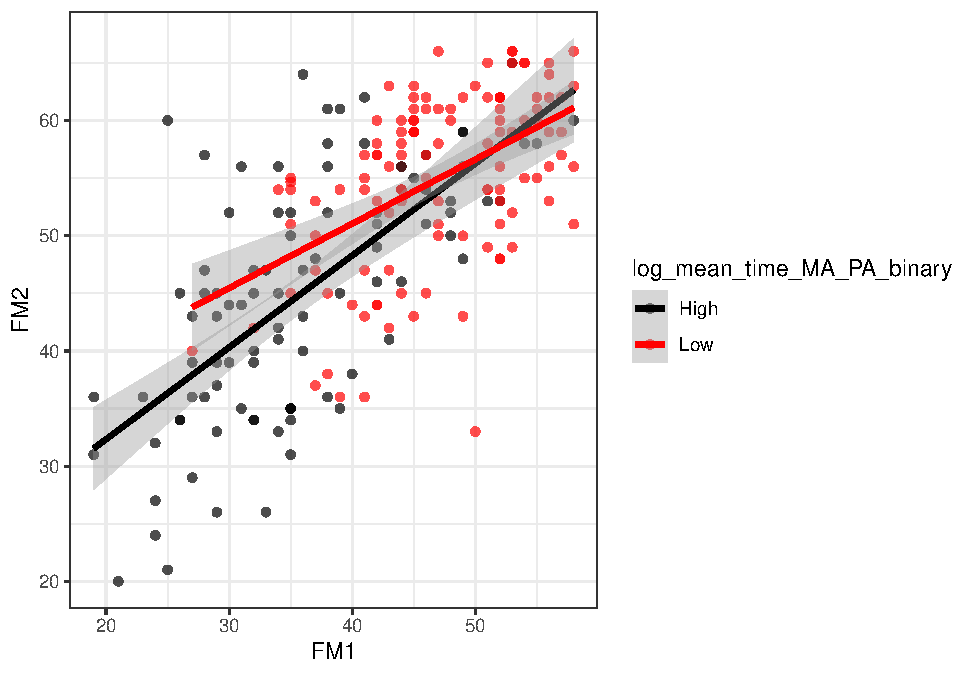
\includegraphics{Final-exam-Pouria_files/figure-latex/unnamed-chunk-6-1.pdf}

However, we see in the linear model that the slope interaction term is
not significant; thus we will see what the new curves are going to look
like if we set \texttt{FM1:log\_mean\_time\_MA\_PA\_binaryLow\ =\ 0} or
equivalently \texttt{lm.fit\$coefficients{[}4{]}\ =\ 0}.

\begin{Shaded}
\begin{Highlighting}[]
\CommentTok{\# Get the coefficients and zero the ones that are not significant }
\CommentTok{\# (p{-}values \textgreater{} .05)}
\NormalTok{coeff }\OtherTok{\textless{}{-}} \FunctionTok{coef}\NormalTok{(}\FunctionTok{summary}\NormalTok{(lm.fit))}
\NormalTok{lm.fit}\SpecialCharTok{$}\NormalTok{coefficients[coeff[,}\DecValTok{4}\NormalTok{]}\SpecialCharTok{\textgreater{}}\NormalTok{.}\DecValTok{05}\NormalTok{] }\OtherTok{=} \DecValTok{0}

\NormalTok{predslm }\OtherTok{=} \FunctionTok{predict}\NormalTok{(lm.fit, }\AttributeTok{interval =} \StringTok{"confidence"}\NormalTok{)}
\NormalTok{datlm }\OtherTok{=} \FunctionTok{cbind}\NormalTok{(data, predslm)}


\FunctionTok{ggplot}\NormalTok{(datlm, }\FunctionTok{aes}\NormalTok{(FM1, }\AttributeTok{y =}\NormalTok{ FM2, }\AttributeTok{color =}\NormalTok{ log\_mean\_time\_MA\_PA\_binary) ) }\SpecialCharTok{+}
  \FunctionTok{geom\_point}\NormalTok{() }\SpecialCharTok{+}
  \FunctionTok{geom\_ribbon}\NormalTok{( }\FunctionTok{aes}\NormalTok{(}\AttributeTok{ymin =}\NormalTok{ lwr, }\AttributeTok{ymax =}\NormalTok{ upr, }
                   \AttributeTok{fill =}\NormalTok{ log\_mean\_time\_MA\_PA\_binary, }\AttributeTok{color =} \ConstantTok{NULL}\NormalTok{), }\AttributeTok{alpha =}\NormalTok{ .}\DecValTok{15}\NormalTok{) }\SpecialCharTok{+}
  \FunctionTok{geom\_line}\NormalTok{( }\FunctionTok{aes}\NormalTok{(}\AttributeTok{y =}\NormalTok{ fit), }\AttributeTok{size =} \DecValTok{1}\NormalTok{) }\SpecialCharTok{+}
  \FunctionTok{scale\_color\_manual}\NormalTok{(}\AttributeTok{values =} \FunctionTok{c}\NormalTok{(}\StringTok{"black"}\NormalTok{, }\StringTok{"red"}\NormalTok{)) }\SpecialCharTok{+}
  \FunctionTok{scale\_fill\_manual}\NormalTok{(}\AttributeTok{values =} \FunctionTok{c}\NormalTok{(}\StringTok{"black"}\NormalTok{, }\StringTok{"red"}\NormalTok{)) }\SpecialCharTok{+}
  \FunctionTok{theme\_bw}\NormalTok{()}
\end{Highlighting}
\end{Shaded}

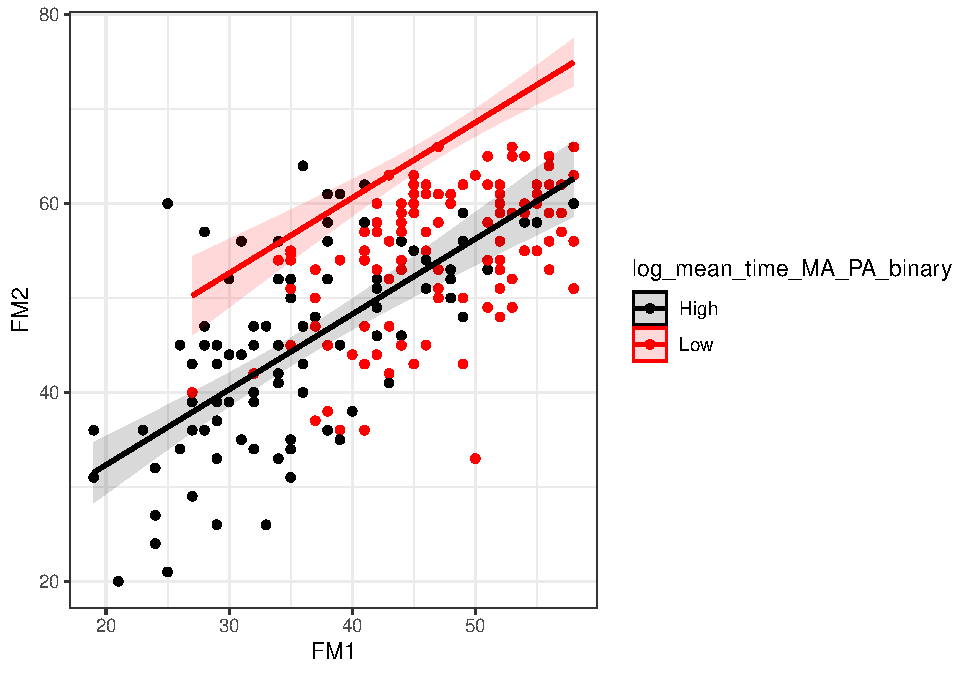
\includegraphics{Final-exam-Pouria_files/figure-latex/unnamed-chunk-7-1.pdf}

\hypertarget{question-2-10-20-points}{%
\section{Question 2 (10 + 20 points)}\label{question-2-10-20-points}}

\textbf{Q2. Estimating regression coefficients CI with a manually
implemented bootstrap. (30 points:: 10 + 20)}

\begin{enumerate}
\def\labelenumi{\arabic{enumi}.}
\tightlist
\item
  Estimate 95\% confidence interval via the ``typical'' least square
  regression.
\end{enumerate}

\begin{enumerate}
\def\labelenumi{\Alph{enumi}.}
\tightlist
\item
  \texttt{set.seed(123)}. Fit a lasso model (with optimal lambda
  according to 1 SE) to predict \texttt{FM2} from the data.
\item
  Perform a ``typical'' regression model (\texttt{lm()}) to predict
  \texttt{FM2} using only the lasso-selected variables. Report the 95\%
  confidence interval of the estimated coefficients using the R output
  (which uses the formulas in the text book).
\end{enumerate}

\begin{enumerate}
\def\labelenumi{\arabic{enumi}.}
\setcounter{enumi}{1}
\tightlist
\item
  Estimate 95\% confidence interval via the bootstrap.
\end{enumerate}

\begin{enumerate}
\def\labelenumi{\Alph{enumi}.}
\item
  \texttt{set.seed(123)}. Now implement a bootstrap ``manually'' (i.e.,
  write the code to do the sampling without any boot function from R) to
  estimate the 95\% confidence interval of the parameters for the
  lasso-selected variables. Plot the histogram of the coefficient
  estimate distribution for \texttt{FM1}. Use percentiles to get the
  95\% CIs for all parameters. Make sure your results do not depend (too
  much) on your number of samples by generating many samples (report
  results for few, many, and even more samples). *Hint: Remember that in
  resampling for boostrapping, replacement is allowed, so use
  \texttt{sample(\textasciitilde{},\textasciitilde{},\ replace=T)}.
\item
  Compare the coefficient estimates and the CIs from both methods -
  \texttt{lm()} and regression and from the bootstrap. Discuss
  similarities/differences in your R notebook (note that any differences
  may be understood by performing regression diagnostics -- remember the
  assumptions of regression
  \texttt{and\ notably\ how\ are\ computed\ the\ regression\ coefficient\ SE\ for\ regression\ using\ formulas\ in\ the\ textbook})
\end{enumerate}

\begin{center}\rule{0.5\linewidth}{0.5pt}\end{center}

\hypertarget{q2.1---a}{%
\subsection{Q2.1 - A}\label{q2.1---a}}

\begin{Shaded}
\begin{Highlighting}[]
\NormalTok{x }\OtherTok{=} \FunctionTok{model.matrix}\NormalTok{ ( FM2}\SpecialCharTok{\textasciitilde{}}\NormalTok{.,data\_final)}
\NormalTok{y}\OtherTok{=}\NormalTok{ data\_final}\SpecialCharTok{$}\NormalTok{FM2}
\end{Highlighting}
\end{Shaded}

\begin{Shaded}
\begin{Highlighting}[]
\CommentTok{\# Finding best lambda}
\FunctionTok{set.seed}\NormalTok{(}\DecValTok{123}\NormalTok{)}
\NormalTok{lasso\_reg }\OtherTok{=} \FunctionTok{cv.glmnet}\NormalTok{(x, y,}\AttributeTok{alpha =} \DecValTok{1}\NormalTok{)}
\FunctionTok{plot}\NormalTok{(lasso\_reg)}
\end{Highlighting}
\end{Shaded}

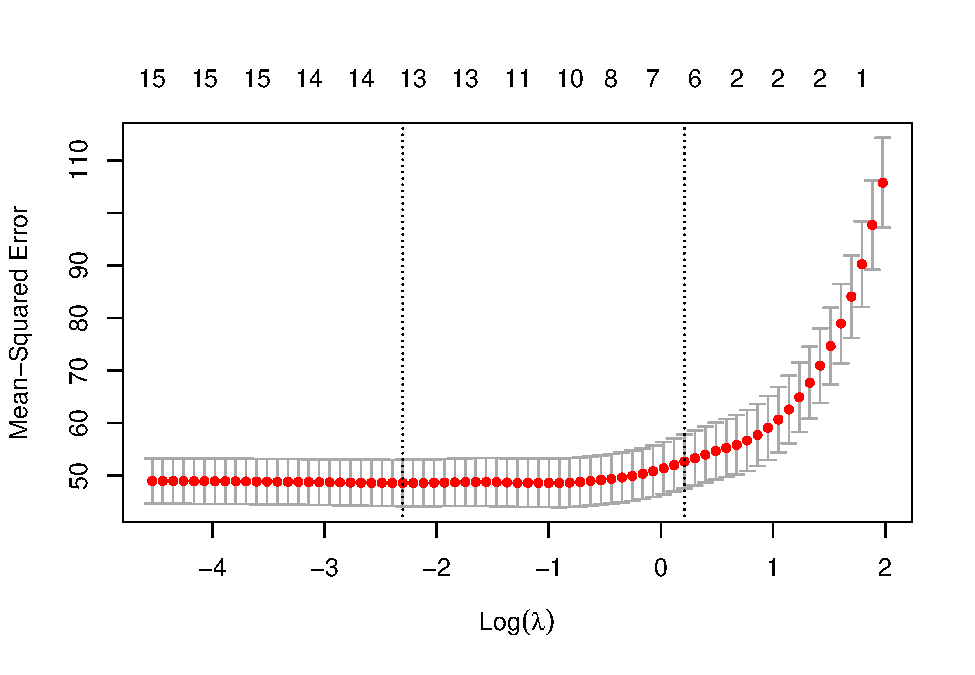
\includegraphics{Final-exam-Pouria_files/figure-latex/unnamed-chunk-9-1.pdf}

\begin{Shaded}
\begin{Highlighting}[]
\NormalTok{bestlam }\OtherTok{=}\NormalTok{lasso\_reg}\SpecialCharTok{$}\NormalTok{lambda}\FloatTok{.1}\NormalTok{se}

\CommentTok{\# Finding coefficients for best lambda}
\NormalTok{out.lasso }\OtherTok{\textless{}{-}} \FunctionTok{glmnet}\NormalTok{(x, y, }\AttributeTok{alpha=}\DecValTok{1}\NormalTok{)}
\NormalTok{lasso.coef }\OtherTok{\textless{}{-}} \FunctionTok{predict}\NormalTok{ (out.lasso , }\AttributeTok{type =} \StringTok{"coefficients"}\NormalTok{, }\AttributeTok{s =}\NormalTok{ bestlam)}
\NormalTok{lasso.coef}
\end{Highlighting}
\end{Shaded}

\begin{verbatim}
## 17 x 1 sparse Matrix of class "dgCMatrix"
##                                1
## (Intercept)         33.851305235
## (Intercept)          .          
## CHAMchallenge        0.005927197
## ave_CAHM             .          
## EQ_index             .          
## SIS_hand             .          
## RNLIadj              0.015732230
## NIHtot               .          
## log_mean_time_MA_PA -1.702129410
## log_mean_time_LA_PA  .          
## grip_MA              0.007451039
## grip_LA              .          
## dose_hours           .          
## onset_to_rand       -0.021135073
## age_at_rand          .          
## old_stroke           .          
## FM1                  0.463499511
\end{verbatim}

\begin{Shaded}
\begin{Highlighting}[]
\NormalTok{coeff}\OtherTok{\textless{}{-}}\NormalTok{ lasso.coef[}\DecValTok{3}\SpecialCharTok{:}\DecValTok{17}\NormalTok{,]}


\NormalTok{selected\_vars }\OtherTok{=} \FunctionTok{names}\NormalTok{(coeff [ coeff }\SpecialCharTok{!=} \DecValTok{0}\NormalTok{ ] )}

\NormalTok{lasso\_df }\OtherTok{=}\NormalTok{ data\_final[,}\FunctionTok{c}\NormalTok{(selected\_vars,}\StringTok{"FM2"}\NormalTok{)]}
\FunctionTok{head}\NormalTok{(lasso\_df)}
\end{Highlighting}
\end{Shaded}

\begin{verbatim}
##   CHAMchallenge RNLIadj log_mean_time_MA_PA grip_MA onset_to_rand FM1 FM2
## 1           100  46.363               3.465   2.000            79  34  42
## 2            50  39.090               3.989   1.333            43  28  45
## 3            50  61.818               0.987   8.666            70  39  36
## 4           100  85.454               0.607  36.666            17  56  64
## 5            90  78.181               2.278   4.666            63  39  45
## 6           100  61.818               3.499   6.000            75  28  36
\end{verbatim}

\hypertarget{q2.1---b}{%
\subsection{Q2.1 - B}\label{q2.1---b}}

\begin{Shaded}
\begin{Highlighting}[]
\CommentTok{\# Fitting linear model}
\NormalTok{lin\_mod }\OtherTok{=} \FunctionTok{lm}\NormalTok{(FM2}\SpecialCharTok{\textasciitilde{}}\NormalTok{., lasso\_df)}
\FunctionTok{summary}\NormalTok{(lin\_mod)}
\end{Highlighting}
\end{Shaded}

\begin{verbatim}
## 
## Call:
## lm(formula = FM2 ~ ., data = lasso_df)
## 
## Residuals:
##      Min       1Q   Median       3Q      Max 
## -18.5060  -4.0220   0.6447   4.2456  17.8227 
## 
## Coefficients:
##                     Estimate Std. Error t value Pr(>|t|)    
## (Intercept)         30.62471    4.82566   6.346 1.37e-09 ***
## CHAMchallenge        0.03484    0.01864   1.869  0.06300 .  
## RNLIadj              0.06663    0.02783   2.394  0.01757 *  
## log_mean_time_MA_PA -2.07288    0.69192  -2.996  0.00307 ** 
## grip_MA              0.05329    0.06164   0.865  0.38830    
## onset_to_rand       -0.06550    0.02315  -2.829  0.00513 ** 
## FM1                  0.45965    0.07894   5.822 2.19e-08 ***
## ---
## Signif. codes:  0 '***' 0.001 '**' 0.01 '*' 0.05 '.' 0.1 ' ' 1
## 
## Residual standard error: 6.868 on 207 degrees of freedom
## Multiple R-squared:  0.5664, Adjusted R-squared:  0.5538 
## F-statistic: 45.06 on 6 and 207 DF,  p-value: < 2.2e-16
\end{verbatim}

\begin{Shaded}
\begin{Highlighting}[]
\CommentTok{\# Checking confidence intervals}
\FunctionTok{confint}\NormalTok{(lin\_mod, }\AttributeTok{level=}\FloatTok{0.95}\NormalTok{)}
\end{Highlighting}
\end{Shaded}

\begin{verbatim}
##                            2.5 %      97.5 %
## (Intercept)         21.110967082 40.13845040
## CHAMchallenge       -0.001905412  0.07158818
## RNLIadj              0.011752841  0.12150262
## log_mean_time_MA_PA -3.436996814 -0.70875779
## grip_MA             -0.068237590  0.17482146
## onset_to_rand       -0.111148324 -0.01985430
## FM1                  0.304007562  0.61528250
\end{verbatim}

\hypertarget{q2.2---a}{%
\subsection{Q2.2 - A}\label{q2.2---a}}

\begin{Shaded}
\begin{Highlighting}[]
\CommentTok{\# Bootstrap}
\FunctionTok{set.seed}\NormalTok{(}\DecValTok{123}\NormalTok{)}
\NormalTok{datalist }\OtherTok{=} \FunctionTok{matrix}\NormalTok{(}\FunctionTok{rep}\NormalTok{(}\DecValTok{0}\NormalTok{,}\DecValTok{10000}\SpecialCharTok{*}\DecValTok{7}\NormalTok{),  }\AttributeTok{ncol =} \DecValTok{7}\NormalTok{)}

\ControlFlowTok{for}\NormalTok{(i }\ControlFlowTok{in} \DecValTok{1}\SpecialCharTok{:}\DecValTok{10000}\NormalTok{)\{}
  \CommentTok{\# sample data}
\NormalTok{  sample\_df }\OtherTok{=}\NormalTok{ lasso\_df[}\FunctionTok{sample}\NormalTok{(}\FunctionTok{nrow}\NormalTok{(lasso\_df), }\FunctionTok{nrow}\NormalTok{(lasso\_df),}\AttributeTok{replace =}\ConstantTok{TRUE}\NormalTok{),] }
\NormalTok{  samp\_lin\_mod }\OtherTok{=} \FunctionTok{lm}\NormalTok{(FM2}\SpecialCharTok{\textasciitilde{}}\NormalTok{., sample\_df)}
\NormalTok{  datalist[i,] }\OtherTok{=}\NormalTok{   samp\_lin\_mod}\SpecialCharTok{$}\NormalTok{coefficients}
\NormalTok{\}}
\CommentTok{\# boots\_values \textless{}{-} dplyr::bind\_rows(datalist)}
\NormalTok{boot.coeff }\OtherTok{\textless{}{-}} \FunctionTok{data.frame}\NormalTok{(datalist) }\SpecialCharTok{\%\textgreater{}\%}
  \FunctionTok{set\_colnames}\NormalTok{(}\FunctionTok{names}\NormalTok{(}\FunctionTok{coefficients}\NormalTok{(lin\_mod)))}
\CommentTok{\# Bootstrap mean and 95p confidence interval}
\FunctionTok{colMeans}\NormalTok{(boot.coeff)}
\end{Highlighting}
\end{Shaded}

\begin{verbatim}
##         (Intercept)       CHAMchallenge             RNLIadj log_mean_time_MA_PA 
##         30.86551320          0.03485211          0.06571602         -2.09231212 
##             grip_MA       onset_to_rand                 FM1 
##          0.05108533         -0.06588801          0.45756524
\end{verbatim}

\begin{Shaded}
\begin{Highlighting}[]
\FunctionTok{apply}\NormalTok{(boot.coeff, }\DecValTok{2}\NormalTok{, }\ControlFlowTok{function}\NormalTok{(x)\{}\FunctionTok{mean}\NormalTok{(x)}\SpecialCharTok{+}\FunctionTok{c}\NormalTok{(}\SpecialCharTok{{-}}\FloatTok{1.96}\NormalTok{,}\FloatTok{1.96}\NormalTok{)}\SpecialCharTok{*}\FunctionTok{sd}\NormalTok{(x)\})}
\end{Highlighting}
\end{Shaded}

\begin{verbatim}
##      (Intercept) CHAMchallenge     RNLIadj log_mean_time_MA_PA     grip_MA
## [1,]    21.47917  -0.003738533 0.005905596          -3.4621430 -0.04961539
## [2,]    40.25186   0.073442750 0.125526445          -0.7224813  0.15178605
##      onset_to_rand       FM1
## [1,]   -0.11217759 0.3104196
## [2,]   -0.01959843 0.6047109
\end{verbatim}

\begin{Shaded}
\begin{Highlighting}[]
\CommentTok{\# linear model mean and 95p confidence interval}
\FunctionTok{coef}\NormalTok{(lin\_mod)}
\end{Highlighting}
\end{Shaded}

\begin{verbatim}
##         (Intercept)       CHAMchallenge             RNLIadj log_mean_time_MA_PA 
##         30.62470874          0.03484138          0.06662773         -2.07287730 
##             grip_MA       onset_to_rand                 FM1 
##          0.05329193         -0.06550131          0.45964503
\end{verbatim}

\begin{Shaded}
\begin{Highlighting}[]
\FunctionTok{confint}\NormalTok{(lin\_mod, }\AttributeTok{level=}\FloatTok{0.95}\NormalTok{)}
\end{Highlighting}
\end{Shaded}

\begin{verbatim}
##                            2.5 %      97.5 %
## (Intercept)         21.110967082 40.13845040
## CHAMchallenge       -0.001905412  0.07158818
## RNLIadj              0.011752841  0.12150262
## log_mean_time_MA_PA -3.436996814 -0.70875779
## grip_MA             -0.068237590  0.17482146
## onset_to_rand       -0.111148324 -0.01985430
## FM1                  0.304007562  0.61528250
\end{verbatim}

Plotting the histogram of the parameter distribution for FM1 resulted
from Bootstrapping:

\begin{Shaded}
\begin{Highlighting}[]
\FunctionTok{ggplot}\NormalTok{(boot.coeff)}\SpecialCharTok{+}
  \FunctionTok{geom\_histogram}\NormalTok{(}\FunctionTok{aes}\NormalTok{(}\AttributeTok{x=}\NormalTok{FM1), }\AttributeTok{bins=}\DecValTok{100}\NormalTok{)}
\end{Highlighting}
\end{Shaded}

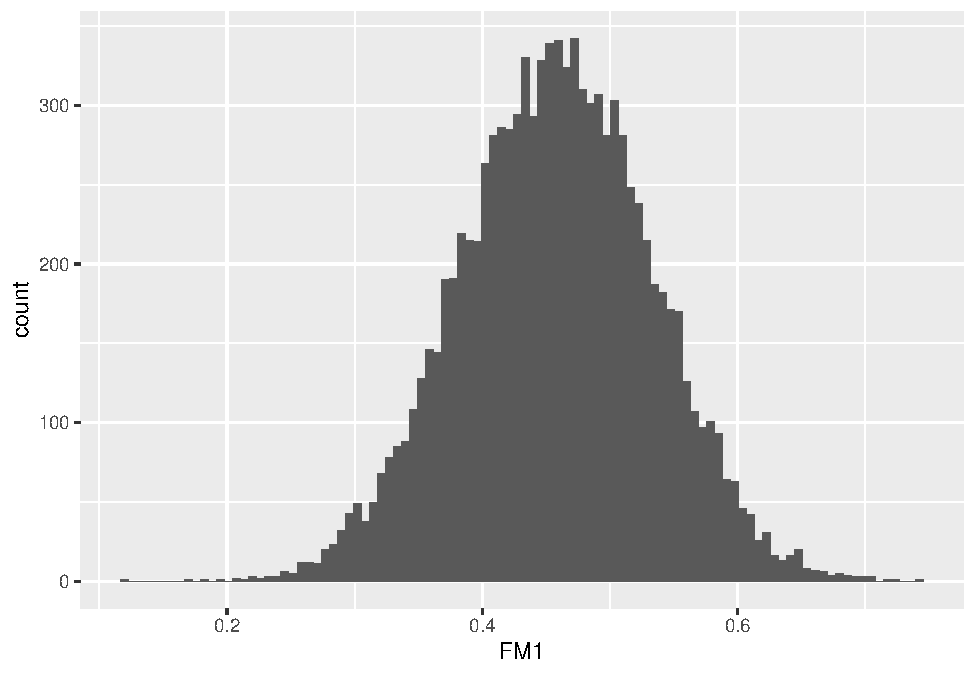
\includegraphics{Final-exam-Pouria_files/figure-latex/unnamed-chunk-15-1.pdf}

\hypertarget{q2.2---b}{%
\subsection{Q2.2 - B}\label{q2.2---b}}

\hypertarget{question-3-25-5}{%
\section{Question 3 (25 + 5)}\label{question-3-25-5}}

\textbf{Q3. Trees and random forest. (30 points: 25 + 5)}

\begin{itemize}
\tightlist
\item
  Divide the data into a training and a test set of 20\% of the data
  assigned to the test. Use \texttt{sample(nrow(.),\ 0.2*nrow(.))}.
\end{itemize}

\begin{enumerate}
\def\labelenumi{\arabic{enumi}.}
\tightlist
\item
\end{enumerate}

\begin{enumerate}
\def\labelenumi{\alph{enumi}.}
\tightlist
\item
  Predict \texttt{FM2} from the data using a pruned tree via
  cross-validation. Plot the tree. Discuss your results.
\item
  Predict \texttt{FM2} using bagging. Discuss your results (including
  variable importance)
\item
  Predict \texttt{FM2} using random forest. Discuss your results.
\item
  Plot the variable importance for random forest. Compare with the
  pruned tree and discuss your results.
\end{enumerate}

\begin{enumerate}
\def\labelenumi{\arabic{enumi}.}
\setcounter{enumi}{1}
\item
  Predict \texttt{FM2} using the lasso model of Q2 with the same test
  set. Then, Compare the MSE on the test set of the four different
  methods.
\item
  Predict \texttt{FM2} using
  \texttt{a\ lasso\ model\ selected\ based\ on\ cross-validation\ and\ using\ the\ same\ test\ set}.
  Then, Compare the MSE on the test set of the four different methods.
\end{enumerate}

\emph{Hint: Recall that prediction is about investigating how well a
model performs on new data, i.e., the test set here}

\hypertarget{q3.1---a}{%
\subsection{Q3.1 - A}\label{q3.1---a}}

\textbf{Tree-based Regression}

First split the data into train/test sets.

\begin{Shaded}
\begin{Highlighting}[]
\CommentTok{\# Creating test and train sets}
\NormalTok{test\_index }\OtherTok{=}\FunctionTok{sample}\NormalTok{(}\FunctionTok{nrow}\NormalTok{(data\_final), }\FloatTok{0.3}\SpecialCharTok{*}\FunctionTok{nrow}\NormalTok{(data\_final))}
\NormalTok{test\_df }\OtherTok{=}\NormalTok{ data\_final[test\_index,]}
\NormalTok{train\_df }\OtherTok{=}\NormalTok{ data\_final[}\SpecialCharTok{{-}}\NormalTok{test\_index,]}

\CommentTok{\# Train tree and predict MSE}
\NormalTok{tree.FM2 }\OtherTok{=}\FunctionTok{tree}\NormalTok{(FM2}\SpecialCharTok{\textasciitilde{}}\NormalTok{. , train\_df)}
\NormalTok{tree.pred}\OtherTok{=}\FunctionTok{predict}\NormalTok{(tree.FM2 ,test\_df )}
\FunctionTok{plot}\NormalTok{(tree.pred ,test\_df}\SpecialCharTok{$}\NormalTok{FM2)}
\end{Highlighting}
\end{Shaded}

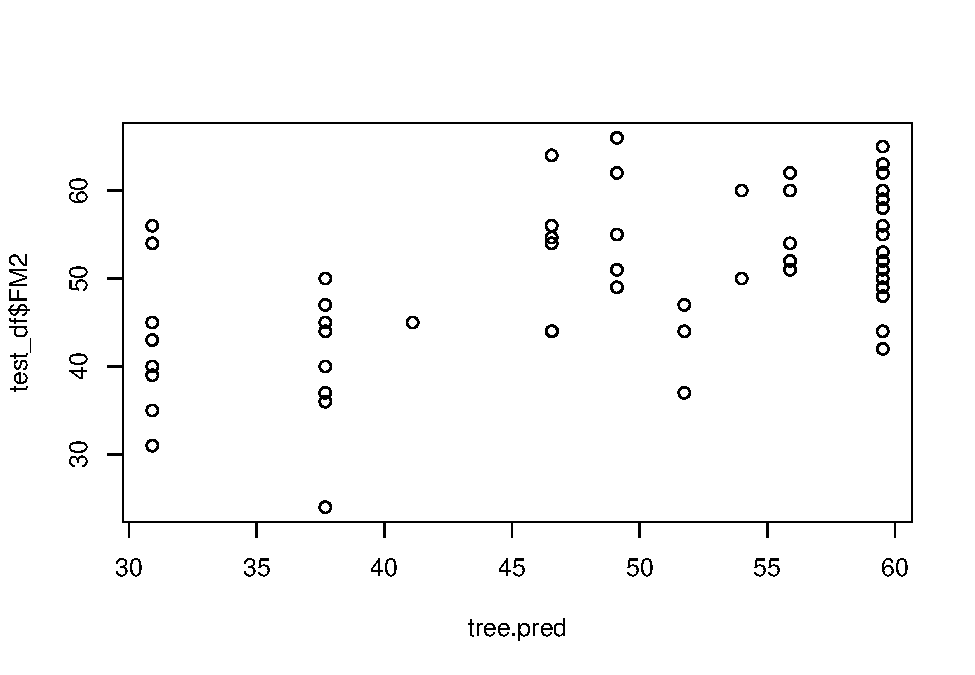
\includegraphics{Final-exam-Pouria_files/figure-latex/unnamed-chunk-16-1.pdf}

Prune the tree

\begin{Shaded}
\begin{Highlighting}[]
\FunctionTok{set.seed}\NormalTok{(}\DecValTok{123}\NormalTok{)}
\NormalTok{cv.FM2 }\OtherTok{=}\FunctionTok{cv.tree}\NormalTok{(tree.FM2 )}
\FunctionTok{plot}\NormalTok{(cv.FM2)}
\end{Highlighting}
\end{Shaded}

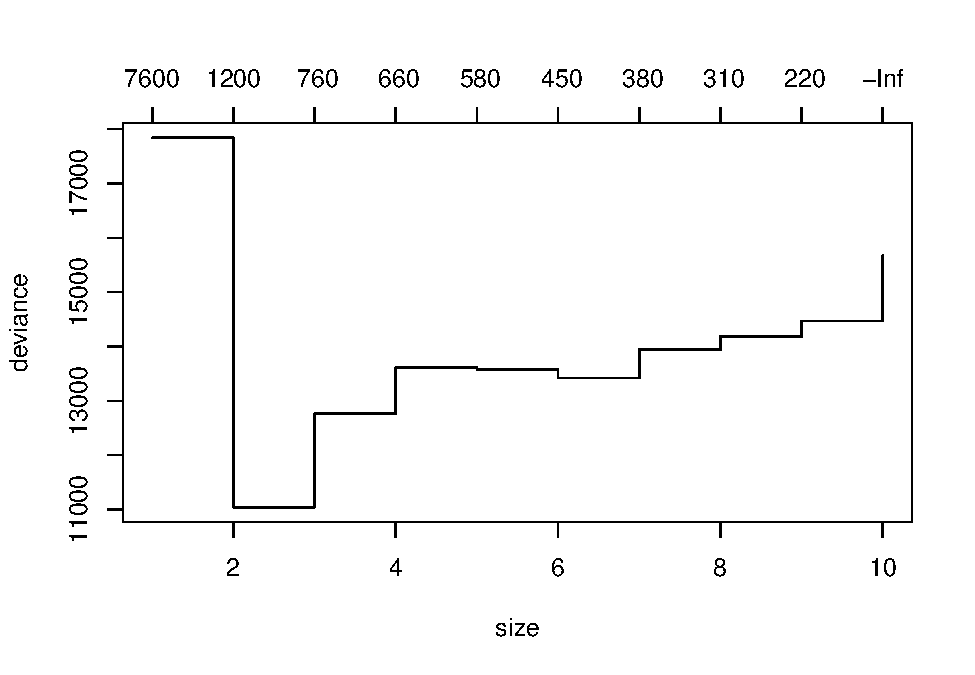
\includegraphics{Final-exam-Pouria_files/figure-latex/unnamed-chunk-17-1.pdf}

\begin{Shaded}
\begin{Highlighting}[]
\NormalTok{prune.FM2 }\OtherTok{=}\FunctionTok{prune.tree}\NormalTok{ (tree.FM2 ,}\AttributeTok{best =}\DecValTok{3}\NormalTok{)}
\FunctionTok{plot}\NormalTok{(prune.FM2 )}
\FunctionTok{text}\NormalTok{(prune.FM2 ,}\AttributeTok{pretty =}\DecValTok{0}\NormalTok{)}
\end{Highlighting}
\end{Shaded}

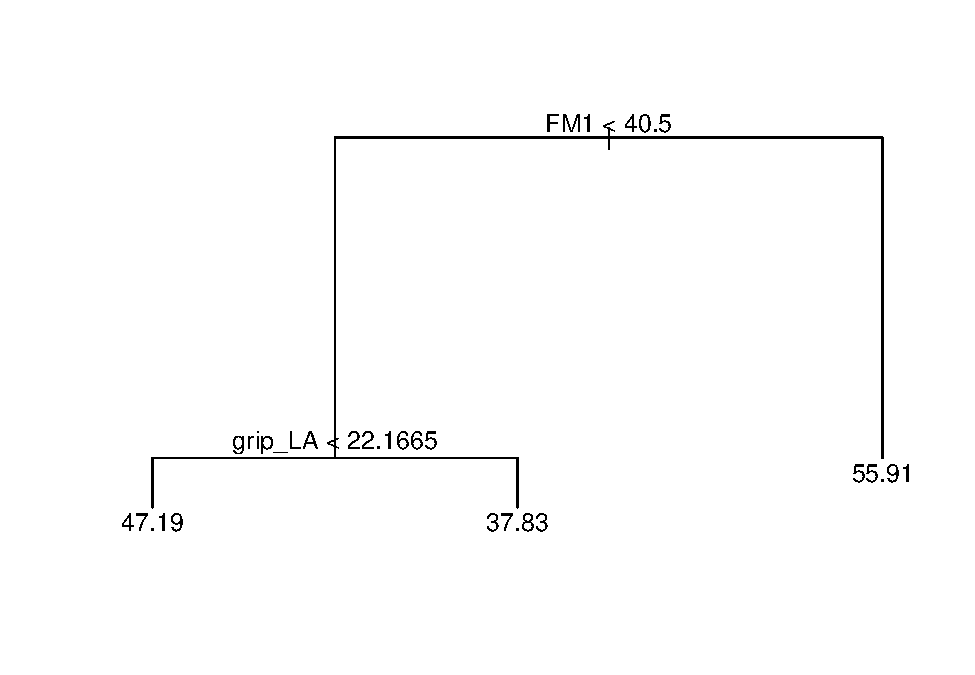
\includegraphics{Final-exam-Pouria_files/figure-latex/unnamed-chunk-17-2.pdf}

Test Error

\begin{Shaded}
\begin{Highlighting}[]
\NormalTok{tree.pred\_prune }\OtherTok{=}\FunctionTok{predict}\NormalTok{(prune.FM2, test\_df)}
\FunctionTok{plot}\NormalTok{(tree.pred\_prune,test\_df}\SpecialCharTok{$}\NormalTok{FM2)}
\end{Highlighting}
\end{Shaded}

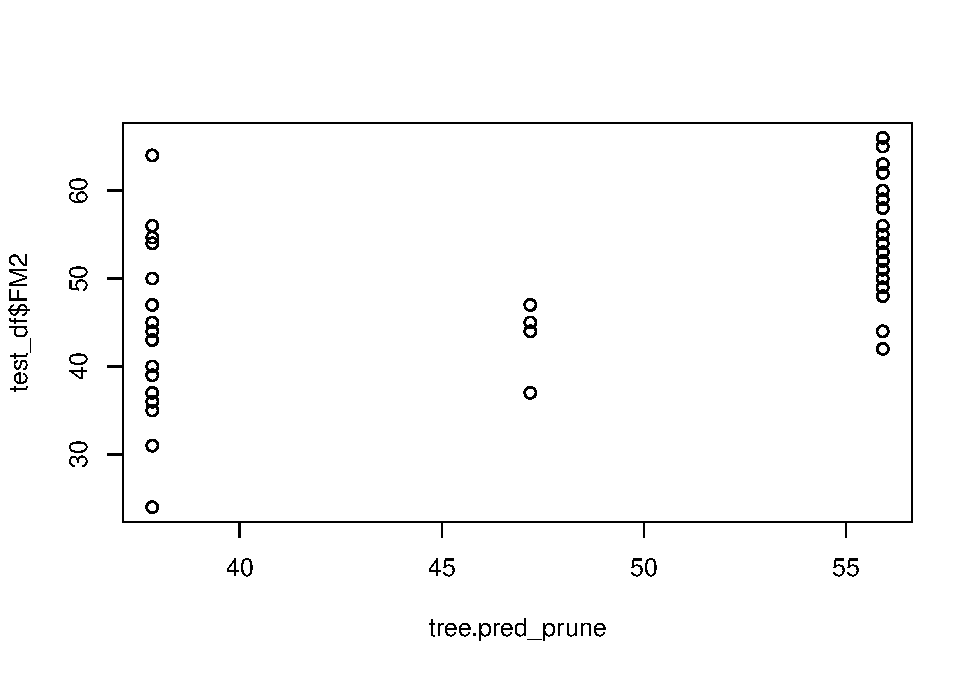
\includegraphics{Final-exam-Pouria_files/figure-latex/unnamed-chunk-18-1.pdf}

\begin{Shaded}
\begin{Highlighting}[]
\NormalTok{MSE\_pruned\_tree }\OtherTok{=} \FunctionTok{mean}\NormalTok{((tree.pred\_prune}\SpecialCharTok{{-}}\NormalTok{test\_df}\SpecialCharTok{$}\NormalTok{FM2)}\SpecialCharTok{\^{}}\DecValTok{2}\NormalTok{)}
\NormalTok{MSE\_pruned\_tree}
\end{Highlighting}
\end{Shaded}

\begin{verbatim}
## [1] 75.17403
\end{verbatim}

\hypertarget{q3.1---b}{%
\subsection{Q3.1 - B}\label{q3.1---b}}

\begin{Shaded}
\begin{Highlighting}[]
\CommentTok{\# Bagging}
\FunctionTok{set.seed}\NormalTok{(}\DecValTok{123}\NormalTok{)}
\NormalTok{bag.FM2 }\OtherTok{=}\FunctionTok{randomForest}\NormalTok{(FM2}\SpecialCharTok{\textasciitilde{}}\NormalTok{.,}\AttributeTok{data=}\NormalTok{train\_df, }\AttributeTok{mtry=}\DecValTok{15}\NormalTok{, }\AttributeTok{importance =}\ConstantTok{TRUE}\NormalTok{)}
\NormalTok{bag.FM2}
\end{Highlighting}
\end{Shaded}

\begin{verbatim}
## 
## Call:
##  randomForest(formula = FM2 ~ ., data = train_df, mtry = 15, importance = TRUE) 
##                Type of random forest: regression
##                      Number of trees: 500
## No. of variables tried at each split: 15
## 
##           Mean of squared residuals: 60.74286
##                     % Var explained: 47.14
\end{verbatim}

\begin{Shaded}
\begin{Highlighting}[]
\NormalTok{yhat.bag }\OtherTok{=} \FunctionTok{predict}\NormalTok{ (bag.FM2 ,}\AttributeTok{newdata =}\NormalTok{test\_df)}
\FunctionTok{plot}\NormalTok{(yhat.bag , test\_df}\SpecialCharTok{$}\NormalTok{FM2)}
\FunctionTok{abline}\NormalTok{ (}\DecValTok{0}\NormalTok{,}\DecValTok{1}\NormalTok{)}
\end{Highlighting}
\end{Shaded}

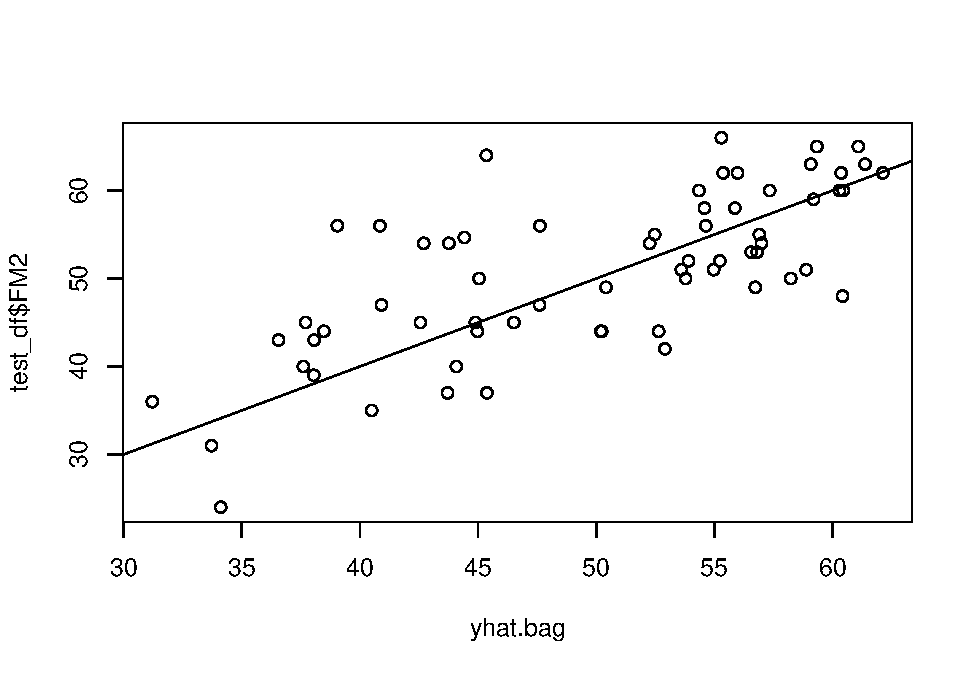
\includegraphics{Final-exam-Pouria_files/figure-latex/unnamed-chunk-20-1.pdf}

\begin{Shaded}
\begin{Highlighting}[]
\NormalTok{MSE\_bagging}\OtherTok{=} \FunctionTok{mean}\NormalTok{(( yhat.bag }\SpecialCharTok{{-}}\NormalTok{test\_df}\SpecialCharTok{$}\NormalTok{FM2)}\SpecialCharTok{\^{}}\DecValTok{2}\NormalTok{)}
\NormalTok{MSE\_bagging}
\end{Highlighting}
\end{Shaded}

\begin{verbatim}
## [1] 44.24469
\end{verbatim}

\hypertarget{q3.1---c}{%
\subsection{Q3.1 - C}\label{q3.1---c}}

\begin{Shaded}
\begin{Highlighting}[]
\CommentTok{\# Random Forest}
\FunctionTok{set.seed}\NormalTok{(}\DecValTok{123}\NormalTok{)}
\NormalTok{RF.FM2 }\OtherTok{=}\FunctionTok{randomForest}\NormalTok{(FM2}\SpecialCharTok{\textasciitilde{}}\NormalTok{.,}\AttributeTok{data=}\NormalTok{train\_df, }\AttributeTok{importance =}\ConstantTok{TRUE}\NormalTok{)}
\NormalTok{RF.FM2}
\end{Highlighting}
\end{Shaded}

\begin{verbatim}
## 
## Call:
##  randomForest(formula = FM2 ~ ., data = train_df, importance = TRUE) 
##                Type of random forest: regression
##                      Number of trees: 500
## No. of variables tried at each split: 5
## 
##           Mean of squared residuals: 56.55222
##                     % Var explained: 50.78
\end{verbatim}

\begin{Shaded}
\begin{Highlighting}[]
\NormalTok{yhat.RF }\OtherTok{=} \FunctionTok{predict}\NormalTok{ (RF.FM2 ,}\AttributeTok{newdata =}\NormalTok{test\_df)}
\FunctionTok{plot}\NormalTok{(yhat.RF , test\_df}\SpecialCharTok{$}\NormalTok{FM2)}
\FunctionTok{abline}\NormalTok{ (}\DecValTok{0}\NormalTok{,}\DecValTok{1}\NormalTok{)}
\end{Highlighting}
\end{Shaded}

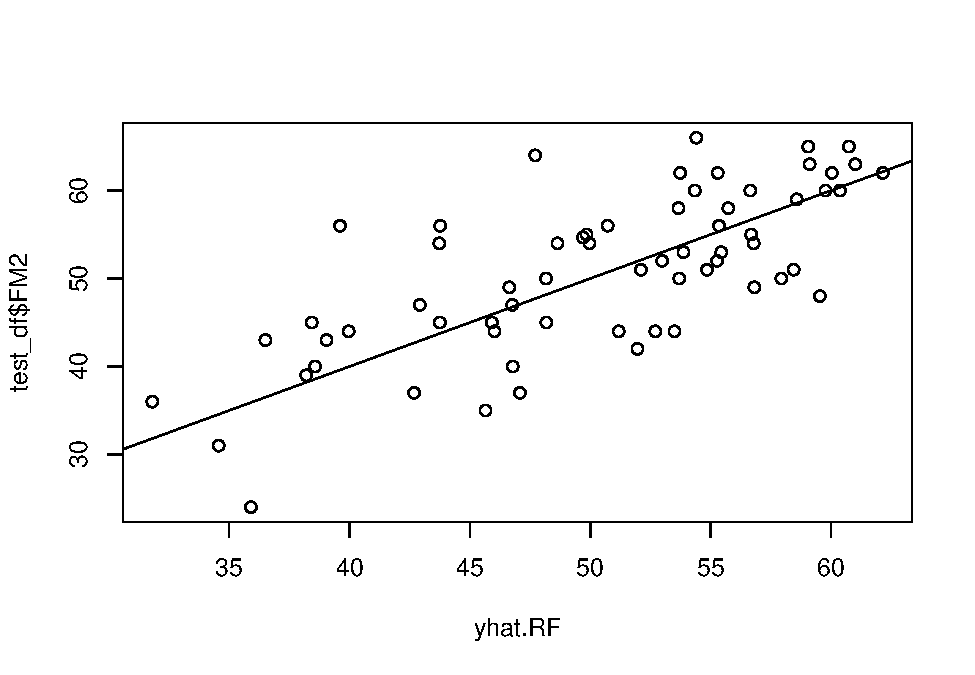
\includegraphics{Final-exam-Pouria_files/figure-latex/unnamed-chunk-23-1.pdf}

\begin{Shaded}
\begin{Highlighting}[]
\NormalTok{MSE\_RF}\OtherTok{=} \FunctionTok{mean}\NormalTok{(( yhat.RF }\SpecialCharTok{{-}}\NormalTok{test\_df}\SpecialCharTok{$}\NormalTok{FM2)}\SpecialCharTok{\^{}}\DecValTok{2}\NormalTok{)}
\NormalTok{MSE\_RF}
\end{Highlighting}
\end{Shaded}

\begin{verbatim}
## [1] 40.95762
\end{verbatim}

\hypertarget{q3.2}{%
\subsection{Q3.2}\label{q3.2}}

\begin{Shaded}
\begin{Highlighting}[]
\FunctionTok{varImpPlot}\NormalTok{(RF.FM2)}
\end{Highlighting}
\end{Shaded}

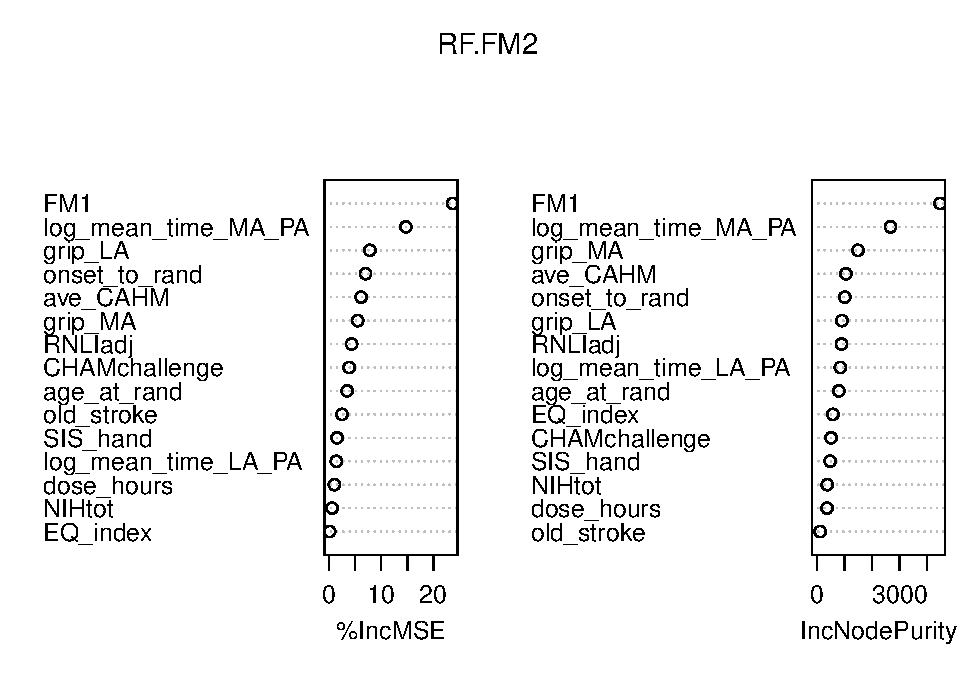
\includegraphics{Final-exam-Pouria_files/figure-latex/unnamed-chunk-25-1.pdf}

\hypertarget{question-4-10-10-10} variable accounted for cut-off, how many
  PCs do you find? Plot the results with a biplot. Discuss your results.
\item
  Now, using K = 2, perform a K-means clustering on the predictor
  variables selected by the lasso.
\item
  Plot the K-means results in the PC1/PC2 axes. Discuss your results.
\end{enumerate}

\begin{Shaded}
\begin{Highlighting}[]
\NormalTok{pr.out }\OtherTok{=} \FunctionTok{prcomp}\NormalTok{(}\FunctionTok{select}\NormalTok{(lasso\_df, }\SpecialCharTok{{-}}\StringTok{"FM2"}\NormalTok{),}\AttributeTok{scale =} \ConstantTok{TRUE}\NormalTok{)}
\NormalTok{variance\_PCS }\OtherTok{=}\NormalTok{(pr.out}\SpecialCharTok{$}\NormalTok{sdev)}\SpecialCharTok{\^{}}\DecValTok{2}\SpecialCharTok{/}\FunctionTok{sum}\NormalTok{((pr.out}\SpecialCharTok{$}\NormalTok{sdev)}\SpecialCharTok{\^{}}\DecValTok{2}\NormalTok{)}
\NormalTok{cumsum\_PCA }\OtherTok{=} \FunctionTok{cumsum}\NormalTok{(variance\_PCS)}

\FunctionTok{ggplot}\NormalTok{() }\SpecialCharTok{+} 
  \FunctionTok{geom\_line}\NormalTok{(}\FunctionTok{aes}\NormalTok{(}\AttributeTok{x =} \DecValTok{1}\SpecialCharTok{:}\FunctionTok{length}\NormalTok{(cumsum\_PCA), }\AttributeTok{y =}\NormalTok{ cumsum\_PCA)) }\SpecialCharTok{+}
  \FunctionTok{geom\_point}\NormalTok{(}\FunctionTok{aes}\NormalTok{(}\AttributeTok{x =} \DecValTok{1}\SpecialCharTok{:}\FunctionTok{length}\NormalTok{(cumsum\_PCA), }\AttributeTok{y =}\NormalTok{ cumsum\_PCA)) }\SpecialCharTok{+}
  \FunctionTok{xlab}\NormalTok{(}\StringTok{"\# PC"}\NormalTok{) }\SpecialCharTok{+} \FunctionTok{ylab}\NormalTok{(}\StringTok{"Cumulative PVE"}\NormalTok{)}
\end{Highlighting}
\end{Shaded}

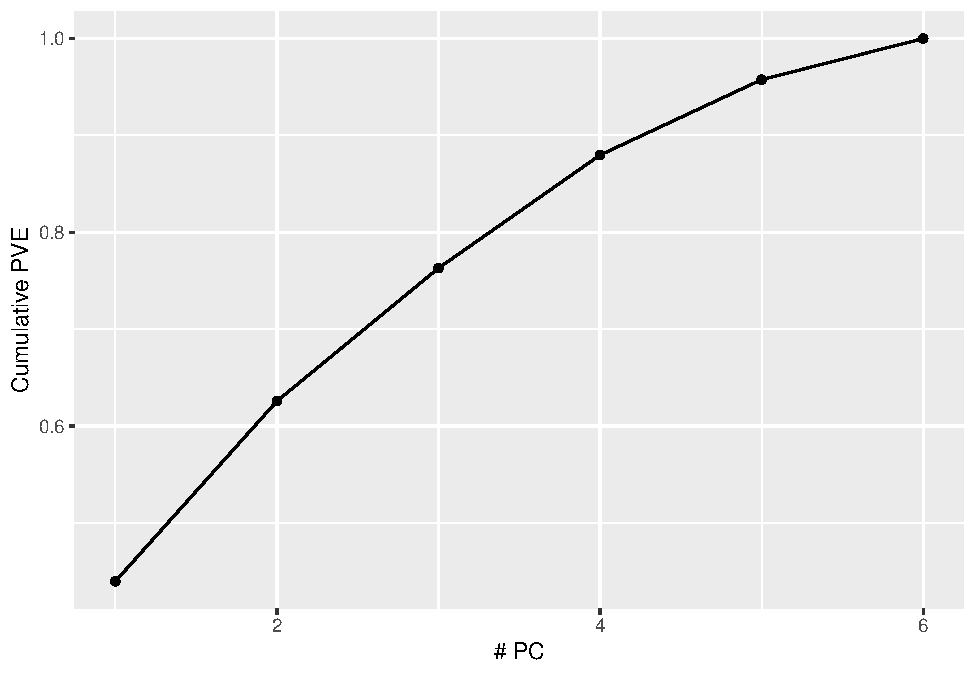
\includegraphics{Final-exam-Pouria_files/figure-latex/unnamed-chunk-26-1.pdf}

\begin{Shaded}
\begin{Highlighting}[]
\CommentTok{\# 5 PCs needed for 90\% variance}
\end{Highlighting}
\end{Shaded}

\begin{Shaded}
\begin{Highlighting}[]
\NormalTok{ggbiplot}\SpecialCharTok{::}\FunctionTok{ggbiplot}\NormalTok{(pr.out)}
\end{Highlighting}
\end{Shaded}

\begin{verbatim}
## Warning: package 'plyr' was built under R version 4.0.5
\end{verbatim}

\begin{verbatim}
## ------------------------------------------------------------------------------
\end{verbatim}

\begin{verbatim}
## You have loaded plyr after dplyr - this is likely to cause problems.
## If you need functions from both plyr and dplyr, please load plyr first, then dplyr:
## library(plyr); library(dplyr)
\end{verbatim}

\begin{verbatim}
## ------------------------------------------------------------------------------
\end{verbatim}

\begin{verbatim}
## 
## Attaching package: 'plyr'
\end{verbatim}

\begin{verbatim}
## The following objects are masked from 'package:dplyr':
## 
##     arrange, count, desc, failwith, id, mutate, rename, summarise,
##     summarize
\end{verbatim}

\begin{verbatim}
## Warning: package 'scales' was built under R version 4.0.5
\end{verbatim}

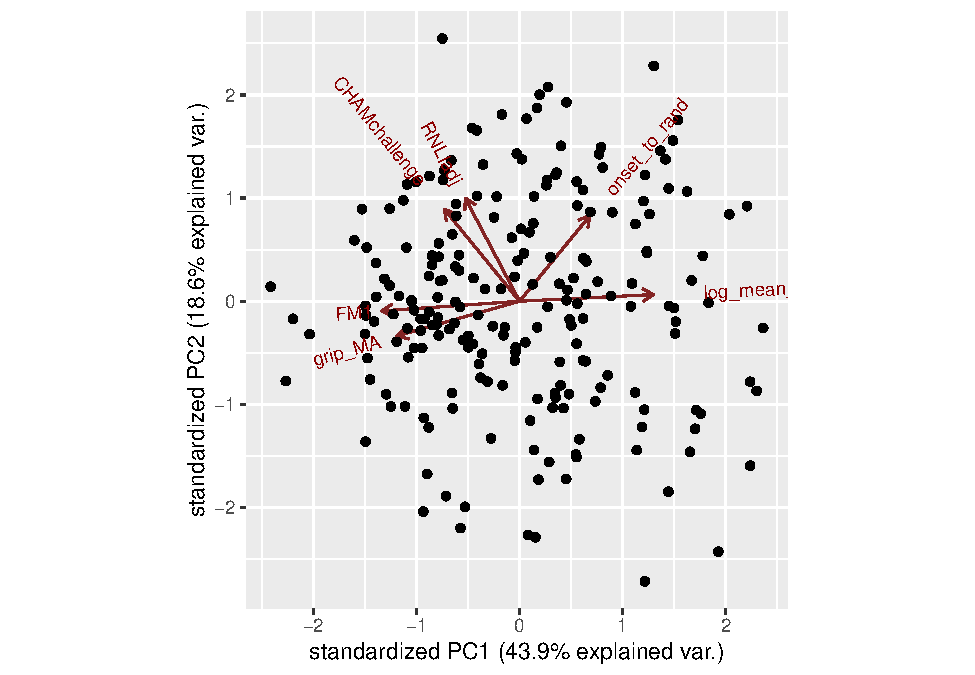
\includegraphics{Final-exam-Pouria_files/figure-latex/unnamed-chunk-27-1.pdf}

\hypertarget{kmeans-clustering-with-k-2}{%
\subsection{Kmeans clustering with k
=2}\label{kmeans-clustering-with-k-2}}

\begin{Shaded}
\begin{Highlighting}[]
\NormalTok{km.out }\OtherTok{=}\FunctionTok{kmeans}\NormalTok{ (}\FunctionTok{select}\NormalTok{(lasso\_df, }\SpecialCharTok{{-}}\StringTok{"FM2"}\NormalTok{),}\DecValTok{2}\NormalTok{, }\AttributeTok{nstart =}\DecValTok{20}\NormalTok{)}
\CommentTok{\# Cluster assignment}
\NormalTok{km.out}\SpecialCharTok{$}\NormalTok{cluster}
\end{Highlighting}
\end{Shaded}

\begin{verbatim}
##   1   2   3   4   5   6   7   8   9  10  11  12  13  14  15  16  17  18  19  20 
##   1   2   2   1   1   1   2   1   1   1   1   2   1   1   2   2   2   1   1   1 
##  21  23  24  25  26  27  28  29  30  31  32  33  34  35  37  38  39  40  41  42 
##   1   1   1   1   1   1   1   1   1   1   1   2   1   1   2   1   1   1   1   2 
##  43  44  45  46  47  48  49  50  51  52  53  54  55  56  57  58  59  60  61  62 
##   1   1   2   1   1   1   1   2   1   1   2   2   1   2   2   1   1   2   1   1 
##  63  64  65  66  67  68  69  70  71  72  73  74  75  76  77  78  79  80  81  82 
##   1   2   2   2   1   2   1   1   2   1   1   1   1   1   1   1   2   2   1   1 
##  83  84  85  86  87  88  89  90  91  93  94  95  96  97  98  99 100 101 102 103 
##   1   1   1   1   2   1   1   1   2   1   1   1   1   1   1   1   1   2   2   1 
## 104 105 106 107 108 109 110 111 112 113 114 115 116 117 118 119 120 121 122 123 
##   2   1   1   1   1   1   1   2   1   2   2   1   2   1   2   2   1   1   2   2 
## 124 125 126 127 128 129 130 131 132 133 134 135 136 137 138 139 140 141 142 143 
##   2   1   1   1   2   2   2   2   2   1   1   2   1   1   1   1   1   1   1   2 
## 144 145 146 147 148 149 150 151 152 153 154 155 156 157 158 159 160 161 162 163 
##   1   1   1   1   1   2   2   1   1   2   2   1   1   2   2   1   1   2   1   1 
## 164 165 166 167 168 170 171 172 173 174 175 176 177 178 179 180 181 182 183 184 
##   1   2   1   2   1   1   1   2   2   1   1   1   2   2   2   1   1   2   1   1 
## 185 186 187 188 189 190 191 192 193 194 195 196 197 198 199 200 201 202 203 204 
##   1   2   2   1   1   2   1   1   1   1   1   1   1   1   1   2   2   1   2   1 
## 205 206 207 208 209 210 211 212 214 215 216 217 218 219 
##   2   1   2   2   2   2   2   1   1   1   2   2   2   1
\end{verbatim}

\hypertarget{plotting-clusters}{%
\subsection{Plotting clusters}\label{plotting-clusters}}

\begin{Shaded}
\begin{Highlighting}[]
\FunctionTok{library}\NormalTok{(factoextra)}
\end{Highlighting}
\end{Shaded}

\begin{verbatim}
## Warning: package 'factoextra' was built under R version 4.0.5
\end{verbatim}

\begin{verbatim}
## Welcome! Want to learn more? See two factoextra-related books at https://goo.gl/ve3WBa
\end{verbatim}

\begin{Shaded}
\begin{Highlighting}[]
\FunctionTok{fviz\_cluster}\NormalTok{(km.out, }\AttributeTok{data =} \FunctionTok{select}\NormalTok{(lasso\_df, }\SpecialCharTok{{-}}\StringTok{"FM2"}\NormalTok{),}
             \CommentTok{\# palette = c("\#2E9FDF", "\#00AFBB", "\#E7B800"), }
             \AttributeTok{geom =} \StringTok{"point"}\NormalTok{,}
             \AttributeTok{ellipse.type =} \StringTok{"convex"}\NormalTok{, }
             \AttributeTok{ggtheme =} \FunctionTok{theme\_bw}\NormalTok{())}
\end{Highlighting}
\end{Shaded}

\includegraphics{Final-exam-Pouria_files/figure-latex/unnamed-chunk-29-1.pdf}

\end{document}
